\documentclass[11pt]{article}
\usepackage[a4paper,margin=25mm]{geometry}
\usepackage{amsmath,amssymb,amsthm,mathtools,booktabs,array,longtable,xcolor,graphicx}
\usepackage[T1]{fontenc}\usepackage{lmodern}
\usepackage[colorlinks=true,linkcolor=teal,citecolor=teal,urlcolor=teal]{hyperref}
\hypersetup{pdftitle={Realization Limits of the Bicomplex Signal Surface},pdfauthor={Akari Hayami (Jian-Yu Huang)},pdfsubject={Successor to Geometric Realization of Bicomplex Signal Manifolds (v11/v12)}}
\graphicspath{{figures/}}
\newtheorem{theorem}{Theorem}[section]
\newtheorem{proposition}[theorem]{Proposition}
\newtheorem{lemma}[theorem]{Lemma}
\newtheorem{corollary}[theorem]{Corollary}
\theoremstyle{definition}\newtheorem{definition}[theorem]{Definition}
\theoremstyle{remark}\newtheorem{remark}[theorem]{Remark}
\newcommand{\R}{\mathbb R}\newcommand{\C}{\mathbb C}\newcommand{\Z}{\mathbb Z}
\newcommand{\Q}{\mathbb Q}\newcommand{\T}{\mathbb T}
\newcommand{\dd}{\,d}\newcommand{\norm}[1]{\left\lVert#1\right\rVert}
\newcommand{\RHom}{\operatorname{RHom}}\newcommand{\End}{\operatorname{End}}\newcommand{\Hom}{\operatorname{Hom}}
\newcommand{\inte}{\operatorname{int}}\newcommand{\orr}{\mathrm{or}}
\DeclareMathOperator{\sgn}{sgn}\DeclareMathOperator{\rank}{rank}
\title{Realization Limits of the Bicomplex Signal Surface:\\
Analytic Rigidity, Smooth Flexibility and Observation Monodromy}
\author{Akari Hayami (Jian-Yu Huang)}
\date{October 2026\\\small Working draft of the corrected successor to
\emph{Geometric Realization of Bicomplex Signal Manifolds} (v11/v12)}
\begin{document}\maketitle
\begin{abstract}
A prescribed power distribution on a two-component signal fixes the moduli of
the components but leaves their phases free. We ask whether this freedom can
realize an explicit ruled surface $S\subset\R^3$ through a fixed readout map.
For the original assignment $(|z_1|^2,|z_2|^2)=(\cos t,1-\cos t)$ the answer
reveals a sharp distinction between analytic and smooth realizations. No
readout that is real-analytic along the circle $\{z_1=0\}$ realizes $S$,
whatever states are used; this excludes affine projections, polynomial maps
and every polynomial in a bicomplex variable and its conjugates. Explicit
$C^\infty$ readouts, however, do exist. The obstruction sits at a single
geometric feature: the two edges of the source are forced onto one circle of
states, while $S$ maps them onto two different lines. Removing that feature
restores analyticity. Each half of the source has a real-analytic readout,
and a modified power assignment has a quadratic one.

We also identify the carriers of the square-root monodromy of the observation
field. It lives on a local system that is indecomposable over $\Z$ and splits
after inverting $2$, and it is distinct from both the fold involution and the
normalization defect. The exceptional pullback of $\Z$ along any continuous
planar map from a convex domain depends only on the domain; folds are seen
instead by the comparison map that defines cohomological smoothness. This
paper supersedes an earlier preprint, whose named statements are reviewed in
an appendix.
\end{abstract}
\tableofcontents

\section{Introduction}\label{sec:intro}
A prescribed power distribution leaves considerable freedom in the phases. We
ask whether this freedom can realize a given surface through a fixed readout.
The surface is the explicit ruled map
\[
 S(t,u)=\bigl(\cos t+2u(1-\cos t),\,(1-u)\sin t,\,u\sqrt{\cos t(2-\cos t)}\bigr),
\]
which the preprint \cite{record} derived from a signal-theoretic picture: a
power-conserving two-component state, its moment map, and a projection onto
three observed coordinates. Its geometry is rich (Figure~\ref{fig:surface}).
It has five cross-cap singularities, an observation field with a topological
dipole, and an explicit $A_3$ residual, and much of this has since been
established rigorously \cite{ruled,stokes}. The realization question itself,
\emph{which states, read out by which maps, actually produce $S$?}, is
answered here. The answer reveals a sharp distinction between analytic
rigidity and smooth flexibility.

\begin{figure}[t]\centering
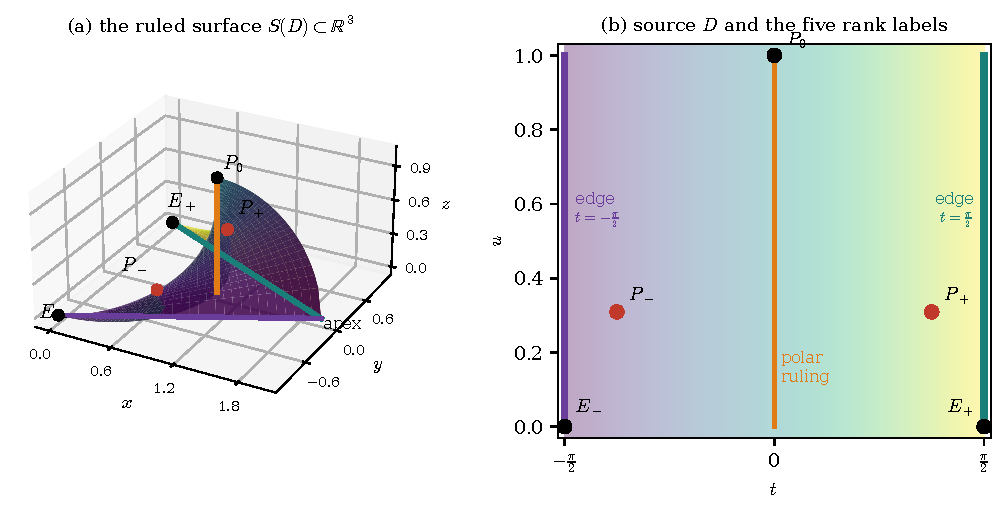
\includegraphics[width=\linewidth]{surface_overview.pdf}
\caption{(a) The ruled surface $S$, coloured by $t$. The two edges
$t=\pm\pi/2$ (teal and purple) lie in the plane $z=0$ and meet at the apex
$(2,0,0)$; the polar ruling $t=0$ (orange) is the vertical segment over
$(1,0)$. (b) The source $D=[-\pi/2,\pi/2]\times[0,1]$ with the five rank
labels of Proposition~\ref{prop:atlas}: the interior cross-caps $P_\pm$, the
boundary half-germ $P_0$ and the corner quarter-germs $E_\pm$.}
\label{fig:surface}
\end{figure}

\paragraph{Main results.}
\begin{enumerate}
\item \emph{Analytic rigidity} (Theorem~\ref{thm:rigidity}). Under the original
assignment $|z_1|^2=\cos t$, every state over the edges $t=\pm\pi/2$ lies on
the circle $C_0=\{z_1=0\}$, while $S$ sends the two edges onto a ``V'' of two
non-collinear segments (Figure~\ref{fig:edges}). A real-analytic image of a
circle cannot contain such a V. Hence no readout that is real-analytic along
$C_0$ realizes $S$ on the closed source. On the source open in $t$ the same
holds for every readout that is real-analytic along $C_0$ and continuous at
the points of $C_0$.
\item \emph{Smooth flexibility and sharpness.}
\begin{itemize}
\item An explicit $C^\infty$ readout realizes $S$ (Theorem~\ref{thm:smooth}).
\item On either half of the source, real-analytic readouts exist, while affine
ones still do not (Proposition~\ref{prop:half}).
\item A different power assignment admits a quadratic readout
(Theorem~\ref{thm:realization}).
\item Readouts that ignore the global phase fail with no regularity hypothesis
at all (Proposition~\ref{prop:gauge}).
\end{itemize}
An edge criterion (Remark~\ref{rem:data}) explains all of these.
\item \emph{Carriers of the monodromy} (Proposition~\ref{prop:carrier}). The
two-traversal restoration of $\sqrt F$ (Figure~\ref{fig:field}) lives on a
rank-two local system that is indecomposable over $\Z$. It differs from the
fold involution and from the normalization defect.
\item \emph{Exceptional pullbacks} (Theorem~\ref{thm:shriek},
Proposition~\ref{prop:detect}). For every continuous map from a convex planar
domain to the plane, $\Psi^!\Z$ is the extension by zero from the interior. Folds
are detected by the smoothness comparison map, whose cokernel is the constant
sheaf on the fold arc.
\end{enumerate}

\paragraph{Organization.} Section~\ref{sec:model} fixes the surface and its
observation field. Section~\ref{sec:realization} proves the rigidity theorem
and its sharpness, and Section~\ref{sec:monodromy} treats the monodromy and
the exceptional pullbacks. Section~\ref{sec:residual} describes the residual
geometry at the cross-caps: a parameter-free $3/4$ resolution law, an
explicit $A_3$ completion, and three different projected curves. The earlier
versions also contained spectral and arithmetic estimates, for Mellin
operators, finite Gram matrices, Hardy evaluation and log-scale windows. They
are classical and independent of the realization question, so we collect them,
in the precise form the model uses, in Appendix~\ref{sec:spectral}, together
with the scope statements that carry over unchanged
(Appendix~\ref{sec:limits}).

\paragraph{Relation to the earlier preprint.} This paper is the corrected
successor of \cite{record}. Appendix~\ref{app:corrections} reviews every named
statement of its final version and records where each is proved, sharpened or
corrected here or in the companion paper \cite{companion}.

\paragraph{The bicomplex model.} We retain ``bicomplex'' as the name of the
model in \cite{record}. Through its idempotent decomposition the bicomplex
algebra is $\C\oplus\C$. Writing an element as a pair $(a,b)$, its three
standard conjugations are $(a,b)\mapsto(\bar a,\bar b)$, $(b,a)$ and
$(\bar b,\bar a)$, which are generated by componentwise conjugation and the
exchange of components. The realization and obstruction theorems below are
therefore statements about two-component complex state families; they do not
require bicomplex multiplication as additional structure. Bicomplex algebra
enters as a natural class of readouts. Every expression built from bicomplex
sums, products, constants and conjugations is a real polynomial map, so this
whole class is covered by Corollary~\ref{cor:excluded}.

\paragraph{Relation to other work.} The completed source atlas, the five rank
singularities, the dipole indices and the fold classification of the planar
observation map were established for the same surface in \cite{ruled,stokes}.
We use them as inputs. The Laplace--Beltrami operator of $S$, its point
interactions at the cross-caps, and the Green, Markov and Krein theory that
replaces earlier operator statements are developed in the companion paper
\cite{companion}, for general surfaces with Whitney cross-caps. The tools used
here are standard: real-analytic functions, smooth partitions of unity,
covering spaces, Verdier duality and mixed Hodge theory. What is new is their
application to this model, which yields the dichotomy and the carrier
classification above.

\section{The surface, its source and the observation field}\label{sec:model}
Throughout,
\begin{equation}\label{eq:S}
 S(t,u)=\bigl(c+2u(1-c),\,(1-u)s,\,uQ\bigr),\qquad
 c=\cos t,\ s=\sin t,\ Q=\sqrt{c(2-c)},
\end{equation}
on the source $D=[-\pi/2,\pi/2]\times[0,1]$. Put
$D_\circ=(-\pi/2,\pi/2)\times[0,1]$ and $D_+=[0,\pi/2]\times[0,1]$. The edges
and the polar ruling map to
\begin{equation}\label{eq:edges}
 S(\pm\tfrac\pi2,u)=(2u,\pm(1-u),0),\qquad S(0,u)=(1,0,u).
\end{equation}
The two edge segments lie on distinct lines through the apex $(2,0,0)$. The
ruling line $\{(1,0,z)\}$ is skew to both edge lines.

\begin{proposition}[Completed source and five rank labels \cite{ruled}]\label{prop:atlas}
Near $t=\epsilon\pi/2$, $\epsilon\in\{1,-1\}$, let $r=Q\geq0$, let
$C(r)=1-\sqrt{1-r^2}$, and put
$B_\epsilon(r,u)=(C+2u(1-C),\epsilon(1-u)\sqrt{1-C^2},ur)$. This extends
analytically to $|r|<1$ and agrees with $S$ on the physical overlap. The
rank-loss labels of the completed source are exactly
\[
 P_0=(0,1),\quad P_\pm=(\pm t_0,u_0),\quad E_\pm=(\pm\pi/2,0),\qquad
 c_0=\tfrac{3-\sqrt5}{2},\ t_0=\arccos c_0,\ u_0=\tfrac{1-c_0}{2}.
\]
Each is a cross-cap of the smooth extension. The adapted determinants are
$\Delta(P_0)=1$, $\Delta(P_\pm)=-5\sqrt{\sqrt5-2}$ and $-\epsilon$ at $E_\pm$.
The physical germs at $P_0$ and $E_\pm$ are a boundary half-germ and corner
quarter-germs.
\end{proposition}
\begin{proof}[Sketch]
$C(r)(2-C(r))=r^2$ gives $C(Q)=c$. Differentiation gives
$(B_\epsilon)_r\times(B_\epsilon)_u=(\epsilon u,2u,0)$ at $r=0$. On $c>0$ the
cross-product equations reduce to $c=1,u=1$, or to $u=(1-c)/2=c(2-c)/2$, that
is $c^2-3c+1=0$. Since $S_{uu}=0$, the cross-cap determinant reduces to
$\det(S_u,S_{ut},S_{tt})$, and the smooth recognition criterion
\cite[Cor.~4.5]{hasegawa} applies. Full proofs, with Lean-checked rank
statements, are in \cite{ruled}.
\end{proof}
The polynomial $c^2-3c+1$ thus picks out the two lateral cross-caps. On
$D_{\rm reg}=D\setminus\{P_0,P_\pm,E_\pm\}$, a connected orientable surface
with corners, $H_1(D_{\rm reg};\Z)=\Z^2$.

\paragraph{The observation field.} On the angular chart $|t|<\pi/2$ the normal
$V=S_t\times S_u$ has components $V_z=N$ and $V_x=M$, where
\begin{equation}\label{eq:F}
 N=(1-c)(1-c-2u),\qquad
 M=\frac{c^2(2-c)-u(1-c+c^2)}{Q},\qquad F=N+iM,\qquad \Psi=(N,M).
\end{equation}
Both components are even in $t$. Since $Q$ vanishes at $t=\pm\pi/2$, the
field $F$ and the planar map $\Psi$ live on $D_\circ$. They depend on the
chart, because reparametrizing the source multiplies $V$ by its Jacobian.

\section{Realizations of the surface by signal states}\label{sec:realization}
Let $S^3=\{z\in\C^2:|z_1|^2+|z_2|^2=1\}$, and let $C_0=\{(0,w):|w|=1\}$ and
$C_1=\{(w,0):|w|=1\}$. The moment map $z\mapsto(|z_1|^2,|z_2|^2)$ sends $S^3$
onto the segment $X+Y=1$. To produce a surface one needs two further pieces
of data: a choice of states over the source, and a map reading those states
out.

\begin{definition}\label{def:realization}
Let $D'\subset D$. A \emph{state family} on $D'$ is any map $z:D'\to S^3$;
continuity is not required. A \emph{readout} is a map $P:U\to\R^3$ on a set
$U\subset\C^2$ containing $z(D')$. The pair \emph{realizes} $S$ if
$P\circ z=S$ on $D'$. The family is \emph{moment-compatible} if
$|z_1(t,u)|^2=\cos t$, as in the original model. A readout is
\emph{real-analytic along $C_0$} if $C_0\subset U$ and $\beta\mapsto P(0,e^{i\beta})$
is real-analytic.
\end{definition}

\subsection{A realization with varying powers}
\begin{theorem}[Quadrature realization]\label{thm:realization}
Put $\zeta_+(t)=e^{it/2}$ and $\zeta_-(t)=\sqrt{1-c/2}+i\sqrt{c/2}$. The state
family and the fixed real quadratic readout
\[
 \Phi(t,u)=\bigl(\sqrt{1-u}\,\zeta_+(t),\ \sqrt u\,\zeta_-(t)\bigr),\qquad
 P(z)=\bigl(\Re z_1^2+|z_2|^2+\Re z_2^2,\ \Im z_1^2,\ \Im z_2^2\bigr)
\]
satisfy $|\Phi_1|^2=1-u$, $|\Phi_2|^2=u$ and $P\circ\Phi=S$ on all of $D$. The
phasors are analytic in the completed charts, and the family is smooth for
$0<u<1$.
\end{theorem}
\begin{proof}
$\zeta_+^2=c+is$ and $\zeta_-^2=1-c+iQ$, so
$P\Phi=((1-u)c+u(2-c),(1-u)s,uQ)=S$. In the edge chart
$t=\epsilon\arccos C(r)$, which is analytic in $r$; so is $\zeta_+$. The
components of $\zeta_-$ become $\sqrt{1-C/2}$ and $r/\sqrt{2(2-C)}$, which are
also analytic.
\end{proof}
The phases encode an orthogonal-circle coupling. This is model data; power
conservation alone does not select it.

\begin{proposition}[Two limits of this realization]\label{prop:twoobs}
(1) No $C^1$ state family can have $|z_2|^2=u$ up to $u=0$, or $|z_1|^2=1-u$ up
to $u=1$.
(2) No three fixed Hermitian $2\times2$ matrices $H_j$ and normalized pure-state
family satisfy $S_j=z^*H_jz$ on $D$.
\end{proposition}
\begin{proof}
(1) At a zero of a $C^1$ component $w$, the derivative of $|w|^2$ is
$2\Re(\overline w\,\partial w)=0$, whereas $\partial_u u=1$.
(2) We have $z^*H_jz=a_j+(Mr(z))_j$, where $r(z)$ is the Bloch vector, a point
of the unit sphere, and $M$ is a real $3\times3$ matrix. If $\rank M\leq2$ the
image is planar, but the values $(1,0,0),(0,1,0),(0,-1,0),(1,0,1)$ of $S$ have
affine determinant $2$. If $M$ is invertible the image is an ellipsoid, which
contains no segment, while $S(0,u)=(1,0,u)$ is one \cite{bloch}.
\end{proof}

\subsection{The original assignment}
Under $|z_1|^2=\cos t$, every state with $t=\pm\pi/2$ lies on $C_0$, and every
state with $t=0$ lies on $C_1$. Both edges are therefore read from a single
circle of states, which a readout must map onto two different lines
(Figure~\ref{fig:edges}). This picture drives the rest of the section.

\begin{figure}[t]\centering
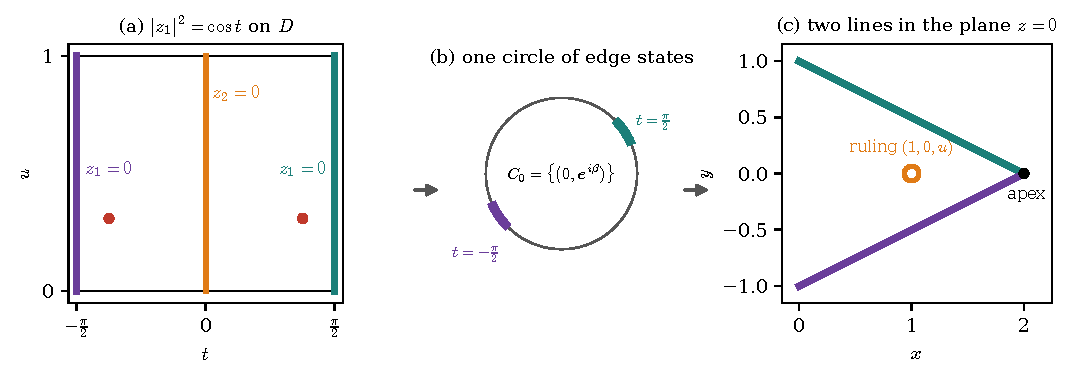
\includegraphics[width=\linewidth]{edge_rigidity.pdf}
\caption{The mechanism behind Theorem~\ref{thm:rigidity}. (a) Under the
original powers, $z_1$ vanishes on both edges and $z_2$ on the polar ruling.
(b) All edge states therefore lie on the circle $C_0$; the arcs shown are
those used by the smooth readout of Theorem~\ref{thm:smooth}. (c) The edges
map to a V in the plane $z=0$, which no analytic image of $C_0$ can contain
(Lemma~\ref{lem:analytic}). The ruling maps onto a segment over $(1,0)$, on a
line skew to both legs.}\label{fig:edges}
\end{figure}
\begin{proposition}[Phase-invariant and mixed-state readouts]\label{prop:gauge}
Suppose $D'$ contains two distinct points of one edge $\{\pm\pi/2\}\times[0,1]$.
No readout with $P(e^{i\gamma}z)=P(z)$ realizes $S$ on $D'$ with a
moment-compatible family. In particular no function of $zz^*$ does, including
any set of Hermitian expectation values. Likewise, for trace-one density
matrices $\rho\geq0$ with $\rho_{11}=\cos t$, no function of $\rho$ realizes $S$.
\end{proposition}
\begin{proof}
$C_0$ is a single orbit of the global phase, so such a readout is constant on
$C_0$, whereas $S$ separates the two edge points. For density matrices,
$|\rho_{12}|^2\leq\rho_{11}\rho_{22}=0$ on the edge, so
$\rho=\mathrm{diag}(0,1)$ there.
\end{proof}

\begin{lemma}[Analytic curves and lines]\label{lem:analytic}
Let $p:J\to\R^3$ be real-analytic on an open interval or on the circle. For
every line $\ell$, either $p(J)\subset\ell$ or $p(J)\cap\ell$ is countable. In
particular $p(J)$ cannot contain uncountable subsets of two distinct lines.
\end{lemma}
\begin{proof}
Choose $x_0\in\ell$ and unit normals $n_1,n_2$ to $\ell$. If
$p(J)\not\subset\ell$, some $n_k\cdot(p-x_0)$ is a nonzero real-analytic
function. Its zero set is discrete, hence countable, and it contains
$p^{-1}(\ell)$. Two distinct lines meet in at most one point.
\end{proof}

\begin{theorem}[Analytic rigidity]\label{thm:rigidity}
Let a moment-compatible family $z$ and a readout $P$ realize $S$ on $D'$.
\begin{enumerate}
\item If $D'=D$, then $P$ is not real-analytic along $C_0$. More generally, $P$
is not real-analytic on any connected open arc of $C_0$ containing all edge
states $z(\pm\pi/2,u)$.
\item If $D'=D_\circ$, $C_0\subset U$ and $P|_{U\cap S^3}$ is continuous at each
point of $C_0$, then $P$ is not real-analytic along $C_0$.
\end{enumerate}
\end{theorem}
\begin{proof}
(1) The image of $C_0$, or of the arc, contains both edge segments of
\eqref{eq:edges}. These are uncountable subsets of distinct lines,
contradicting Lemma~\ref{lem:analytic}.
(2) Fix $u$ and $\epsilon=\pm1$, and take $t_n\to\epsilon\pi/2$. Since
$|z_1(t_n,u)|^2=\cos t_n\to0$, a subsequence of $z(t_n,u)\in S^3$ converges to
some $z^*\in C_0$. Continuity gives $P(z^*)=\lim S(t_n,u)=S(\epsilon\pi/2,u)$,
so both edge segments lie in $P(C_0)$, and part (1) applies.
\end{proof}

\begin{corollary}[Excluded readouts]\label{cor:excluded}
Under the original assignment on $D$ or $D_\circ$, $S$ is not realized by any of
the following:
\begin{itemize}
\item an affine map $\R^4\to\R^3$;
\item a real polynomial map, or a polynomial in a bicomplex variable and its
conjugates;
\item a map that is real-analytic on a neighbourhood of $C_0$.
\end{itemize}
On $D$ this also excludes stereographic projection from a point of $C_0$ that
avoids the edge states. In particular, the ``geometric projection'' of v12
Definition~3.1 cannot be taken from any of these classes.
\end{corollary}

\subsection{Sharpness}
The obstruction is analytic rather than topological: smooth readouts exist.
The construction below reads the ruling parameter $u$ from a phase. Near the
edges $c=0$ it reads $u$ from the phase of $z_2$; near the polar ruling $c=1$
it reads $u$ from the phase of $z_1$. Smooth cutoffs in $c=|z_1|^2$ switch
between these decoders (Figure~\ref{fig:readout}). Table~\ref{tab:decoders}
records why every decoder is smooth wherever it is used.

\begin{figure}[t]\centering
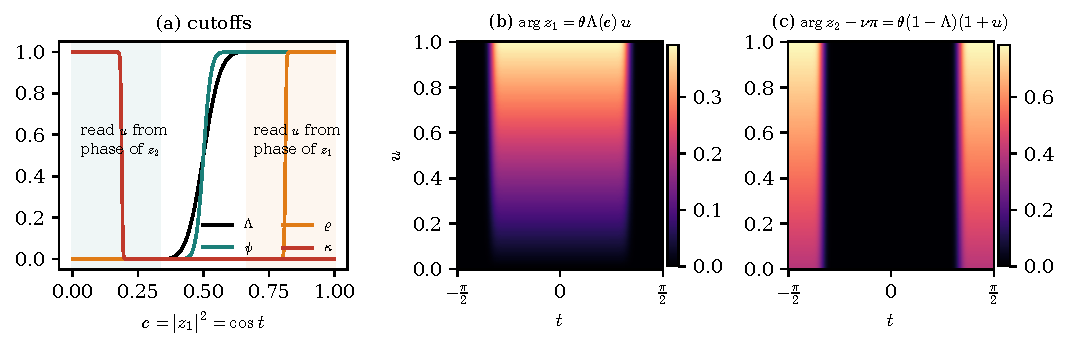
\includegraphics[width=\linewidth]{smooth_readout.pdf}
\caption{The switching readout of Theorem~\ref{thm:smooth}. (a) The cutoffs, as
functions of $c=|z_1|^2$. Near the edges ($c$ small) the ruling parameter $u$
is stored in the phase of $z_2$; near the polar ruling ($c$ close to $1$) it is
stored in the phase of $z_1$. (b), (c) The two phases over the source; each is
monotone in $u$ wherever its decoder is used.}\label{fig:readout}
\end{figure}

\begin{theorem}[$C^\infty$ realization]\label{thm:smooth}
Put $\theta=\pi/8$. Take smooth functions $\Lambda,\psi,\varrho,\kappa:[0,1]\to[0,1]$
such that:
\begin{itemize}
\item $\Lambda=0$ on $[0,\frac14]$, $\Lambda=1$ on $[\frac34,1]$, and $\Lambda$ is
strictly increasing in between;
\item $\psi=0$ on $[0,\frac13]$ and $\psi=1$ on $[\frac23,1]$;
\item $\varrho=0$ on $[0,\frac34]$ and $\varrho=1$ on $[\frac78,1]$;
\item $\kappa=1$ on $[0,\frac18]$ and $\kappa=0$ on $[\frac14,1]$.
\end{itemize}
Let $\chi$ be a smooth $2\pi$-periodic function equal to $1$ on
$[-\frac\pi8,\frac{3\pi}8]$ and to $-1$ on $[\frac{7\pi}8,\frac{11\pi}8]$, and
let $\nu=0$ for $t\geq0$ and $\nu=1$ for $t<0$. Define
\[
 z(t,u)=\bigl(\sqrt c\,e^{i\theta\Lambda(c)u},\
 \sqrt{1-c}\,e^{i(\nu\pi+\theta(1-\Lambda(c))(1+u))}\bigr).
\]
This is a moment-compatible family. It is continuous on $D$, smooth on
$D_\circ$, and smooth up to $t=\pm\pi/2$ in the edge charts, since there
$\sqrt{C(r)}=r/\sqrt{1+\sqrt{1-r^2}}$. With $c=|z_1|^2$ and principal arguments,
set
\begin{gather*}
 \mathcal U=\psi(c)\frac{\arg z_1}{\theta\Lambda(c)}
 +(1-\psi(c))\Bigl(\frac{\arg z_2^2}{2\theta(1-\Lambda(c))}-1\Bigr),\\
 \Sigma=\varrho(c)\,\Re z_2\sqrt{1+c}+(1-\varrho(c))\,|z_2|\chi(\arg z_2)\sqrt{1+c},\\
 \mathcal Q=\kappa(c)\,\Re z_1\sqrt{2-c}+(1-\kappa(c))\sqrt{c(2-c)},
\end{gather*}
where each summand is read as zero where its cutoff vanishes. Then
$P=(|z_1|^2+2\,\mathcal U|z_2|^2,\ (1-\mathcal U)\Sigma,\ \mathcal U\mathcal Q)$
is smooth on an open neighbourhood of $z(D)$, and $P\circ z=S$ on $D$. Hence $S$
has a $C^\infty$ readout defined on all of $\C^2$.
\end{theorem}

\begin{table}[ht]\centering\small\renewcommand{\arraystretch}{1.45}
\begin{tabular}{>{\raggedright\arraybackslash}p{.22\linewidth}>{\raggedright\arraybackslash}p{.19\linewidth}>{\raggedright\arraybackslash}p{.36\linewidth}>{\raggedright\arraybackslash}p{.11\linewidth}}\toprule
Decoder & Used where & Why it is smooth there & Value on the states\\\midrule
$\arg z_1/(\theta\Lambda)$ & $\psi>0$, so $c>\frac13$ & $\Lambda>0$ and $z_1\neq0$; $\arg z_1\in[0,\theta]$ & $u$\\
$\arg z_2^2/(2\theta(1-\Lambda))-1$ & $\psi<1$, so $c<\frac23$ & $\Lambda<1$ and $|z_2|^2>\frac13$; $\arg z_2^2\in[0,\frac\pi2]$ & $u$\\
$\Re z_2\sqrt{1+c}$ & $\varrho>0$, so $c>\frac34$ & smooth; here $\Lambda=1$, so $z_2$ is real & $s$\\
$|z_2|\chi(\arg z_2)\sqrt{1+c}$ & $\varrho<1$, so $c<\frac78$ & $|z_2|^2>\frac18$; $\arg z_2$ lies in a plateau of $\chi$ & $s$\\
$\Re z_1\sqrt{2-c}$ & $\kappa>0$, so $c<\frac14$ & smooth; here $\Lambda=0$, so $z_1=\sqrt c$ & $Q$\\
$\sqrt{c(2-c)}$ & $\kappa<1$, so $c>\frac18$ & $0<c<2$ & $Q$\\\bottomrule
\end{tabular}
\caption{The six decoders of Theorem~\ref{thm:smooth}. Wherever a cutoff is
positive, its decoder is smooth on a neighbourhood of the states there and
takes the listed value.}
\label{tab:decoders}
\end{table}

\begin{proof}[Proof of Theorem~\ref{thm:smooth}]
For $c\geq\frac34$ we have $\Lambda=1$, so
$z_2=\sgn(t)\sqrt{1-\cos t}=\sqrt2\sin(t/2)$, which is smooth; at $t=\pm\pi/2$
only $\sqrt c\to0$ enters. On the states,
$\arg z_1=\theta\Lambda u$, $\arg z_2^2=2\theta(1-\Lambda)(1+u)$, and
$\arg z_2\in\nu\pi+[0,\pi/4]$. Table~\ref{tab:decoders} follows directly: each
decoder takes the stated value wherever its cutoff is nonzero. In the third and
fourth rows, $\Re z_2\sqrt{1+c}=\sgn(t)\sqrt{1-c^2}=s$ and
$\chi(\arg z_2)=\sgn t$.

For smoothness, each summand is defined on the union of two open sets. On the
first its decoder is smooth. On the second its cutoff, a smooth function of
$|z_1|^2$, vanishes identically. The two definitions agree on the overlap, and
the union contains $z(D)$. Hence $P$ is smooth on an open set $U\supset z(D)$,
and substitution gives $P\circ z=S$. Since $z(D)$ is compact, choose an open
$V$ with $z(D)\subset V$ and $\overline V\subset U$ compact, and a smooth bump equal
to $1$ on $V$ and supported in $U$. Its product with $P$ is a $C^\infty$
readout on $\C^2$.
\end{proof}
On $C_0$ this readout traces the two legs of the V on the two disjoint arcs of
Figure~\ref{fig:edges}(b), and the plateau function $\chi$ switches between
them. This is exactly the flexibility that analytic readouts lack.

\begin{lemma}[Analytic retraction]\label{lem:retraction}
Let $M$ be a real-analytic surface without boundary, $z:M\to\R^4$ a
real-analytic immersion, and $K\subset M$ a compact set on which $z$ is
injective. Then there are an open $M'\supset K$ on which $z$ is an embedding,
an open tube $T\supset z(K)$, and a real-analytic map $\varpi:T\to M'$ with
$\varpi\circ z=\mathrm{id}$ near $K$.
\end{lemma}
\begin{proof}
If $z$ were not injective on any neighbourhood of $K$, there would be
$x_n\neq y_n$ with $z(x_n)=z(y_n)$ and both sequences accumulating on $K$. Any
limits $x,y$ satisfy $z(x)=z(y)$, so $x=y$, which contradicts local injectivity
of an immersion near $x$. Shrink to a relatively compact $M'$, on which $z$ is
then an embedding onto $\Sigma=z(M')$. Gram--Schmidt applied to an analytic
local frame gives analytic normal frames, so the normal bundle of $\Sigma$ is
real-analytic. The map $E(x,n)=x+n$ is real-analytic with invertible
differential along the zero section, hence a local analytic diffeomorphism
there \cite{krantzparks}. Compactness gives injectivity on
$\{|n|<\delta\}$ over a neighbourhood of $z(K)$. Put
$\varpi=z^{-1}\circ\mathrm{pr}\circ E^{-1}$.
\end{proof}

\begin{proposition}[One half of the source]\label{prop:half}
(1) If $D'$ contains at least three points of the ruling $\{0\}\times[0,1]$
and at least three points of one edge, no affine readout realizes $S$ on $D'$
with a moment-compatible family. This applies in particular to $D_+$, which
contains the single interior cross-cap $P_+$.
(2) On $D_+$ there are a real-analytic moment-compatible family and a readout,
real-analytic on a neighbourhood of its image, that realize $S$.
\end{proposition}
\begin{proof}
(1) Write $P=b+L$. On $C_1$ the readout traces an ellipse centred at $b$,
possibly degenerate, through three collinear points of the ruling line. A
nondegenerate ellipse meets a line in at most two points, so the ellipse is a
segment and $b$ lies on the ruling line. The same argument on $C_0$ puts $b$
on the edge line, but the two lines are skew.

(2) The closed half source has corners, so we work on an open analytic
surface $M$ containing it. $M$ is glued from the angle chart
$(-\delta,\pi/2)\times(-\delta,1+\delta)$ and the edge chart
$(-\delta,\delta)\times(-\delta,1+\delta)$ in $(r,u)$; there $S$ extends
analytically. Fix $0<\theta<\pi$ and put $z=e^{i\theta u}v$ with
$v=(\sqrt{\cos t},\sqrt2\sin(t/2))$; in the edge chart
$v=(r/\sqrt{1+\sqrt{1-r^2}},(1-r^2)^{1/4})$. Both expressions are analytic on
$M$, and $|z_1|^2=\cos t$ on $D_+$. Since $\partial_uz=i\theta z$ and
$\partial_tz=e^{i\theta u}v'$ with $v'$ real and nonzero, $z$ is an immersion.
It is injective on $D_+$: if $e^{i\theta u}v=e^{i\theta u'}v'$ with $v,v'$
nonnegative, the phase quotient is positive, so $u=u'$ and $t=t'$.
Lemma~\ref{lem:retraction} with $K=D_+$ gives $\varpi$, and $S\circ\varpi$ is
the required readout.
\end{proof}

\begin{remark}[An edge criterion]\label{rem:data}
Lemma~\ref{lem:analytic} gives a simple test for any power assignment
$w=|z_1|^2$. An analytic readout needs $S(w^{-1}(0))$ to lie in the image of an
analytic loop, and a phase-invariant readout needs it to be a single point. The
same holds for $1-w$.

The assignment of Theorem~\ref{thm:realization} passes this test. Its vanishing
edges $u=1$ and $u=0$ map to arcs of the circles $(x-1)^2+z^2=1$ and
$x^2+y^2=1$, and its readout maps the two vanishing circles onto exactly these
circles. The original assignment fails, because $w^{-1}(0)$ consists of both
edges.

A realization of the original model therefore needs one ingredient beyond
the moment map:
\begin{itemize}
\item a non-analytic switching readout, as in Theorem~\ref{thm:smooth};
\item a half source, which keeps one cross-cap and loses the reflection pairing
$S(t,1)=S(-t,1)$; or
\item different powers.
\end{itemize}
Polynomial readouts can approximate $S$ uniformly to any accuracy, by the
Weierstrass theorem applied to Theorem~\ref{thm:smooth}, but never exactly.
Whether a quadratic readout exists on $D_+$ is an interesting open question.
\end{remark}

\section{Observation monodromy and its carriers}\label{sec:monodromy}
\subsection{Interior dipole and square-root restoration}
\begin{theorem}[Dipole and two-traversal restoration]\label{thm:dipole}
The zeros of $F$ in $D_\circ$ are $P_\pm$ and the boundary point $(0,1)$. With
the $(t,u)$ orientation \cite{ruled},
\[
 \det DF(P_\pm)=\mp\frac{5s_0(1-c_0)^2}{Q_0},\qquad\operatorname{Ind}(P_\pm)=\mp1.
\]
Every continuous branch of
$\sqrt F$ transported round a small positive loop about either point changes
sign; two traversals restore it.
\end{theorem}
\begin{proof}
$N=0$ exactly on $c=1$ and on $u=(1-c)/2$. On the first, $M=1-u$. On the
second, $M$ is a positive multiple of $-(c^2-3c+1)$. The determinant follows
from $c_0^2=3c_0-1$, and a nondegenerate zero has small-circle winding equal
to the sign of its determinant. Write $F(\gamma(s))=\exp L(s)$ with a
continuous logarithm, so that $L(1)=L(0)+2\pi in$ with $n=\pm1$. Then
$\chi=\exp(L/2)$ satisfies $\chi(1)=-\chi(0)$, and any other continuous root
differs from $\chi$ by a constant sign.
\end{proof}
The restoration is topological: it counts traversals.
Proposition~\ref{prop:carrier} identifies the structure that carries it. Two
numerical values are worth separating. The Jacobian modulus is
$|\det DF(P_\pm)|\approx2.245$. The value $\sqrt5$, by contrast, is
$|P'(c_0)|$ for the monic polynomial $P(c)=c^2-3c+1$. Both $N$ and $M$ are even
in $t$; the opposite signs of the two determinants come from the $t$-derivatives.

\begin{figure}[t]\centering
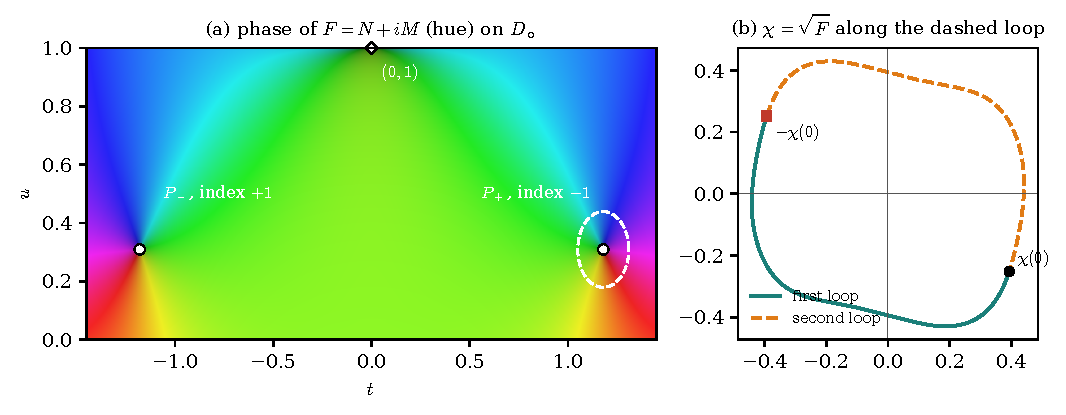
\includegraphics[width=\linewidth]{observation_field.pdf}
\caption{(a) The phase of the observation field $F$ on $D_\circ$, shown for
$|t|\leq1.45$, with the cyclic colour scale on the right; brightness increases
with $|F|$. Every colour meets $P_\pm$, the dipole of
Theorem~\ref{thm:dipole}. (b) A continuous square root $\chi$ of $F$ along the
positively oriented dashed loop about $P_+$, with arrows in the direction of
travel: one traversal ends at $-\chi(0)$, two traversals restore $\chi(0)$.}\label{fig:field}
\end{figure}

\subsection{The polar fold}
\begin{proposition}[Polar fold]\label{prop:polar}
The smooth extension of $\Psi$ at $P_0=(0,1)$ is a Whitney fold of local degree
zero.
\end{proposition}
\begin{proof}
Use the source coordinates $a=-M$ and $b=2\sin(t/2)\sqrt{u-(1-\cos t)/2}$, and
the target coordinates $(N,M)\mapsto(-M,-N)$. The derivative matrix at $(0,1)$
is invertible, and the exact identity $-N=b^2$ gives the normal form $(a,b^2)$.
Reflecting $b$ pairs preimages of opposite orientation.
\end{proof}
The exact charts make the conclusion independent of Taylor remainders; the
remainder displayed in v12 omitted the term $M(t,1)=-t^4/2+O(t^6)$. The full
interior critical locus of $\Psi$ consists of two parts \cite[Thm.~2.4]{stokes}:
the symmetry segment $t=0$, which is an ordinary fold for $u>0$; and a rational
branch, which consists of ordinary folds away from $(0,0)$, where the
ordinary-fold condition fails (Figure~\ref{fig:folds}).

\begin{figure}[t]\centering
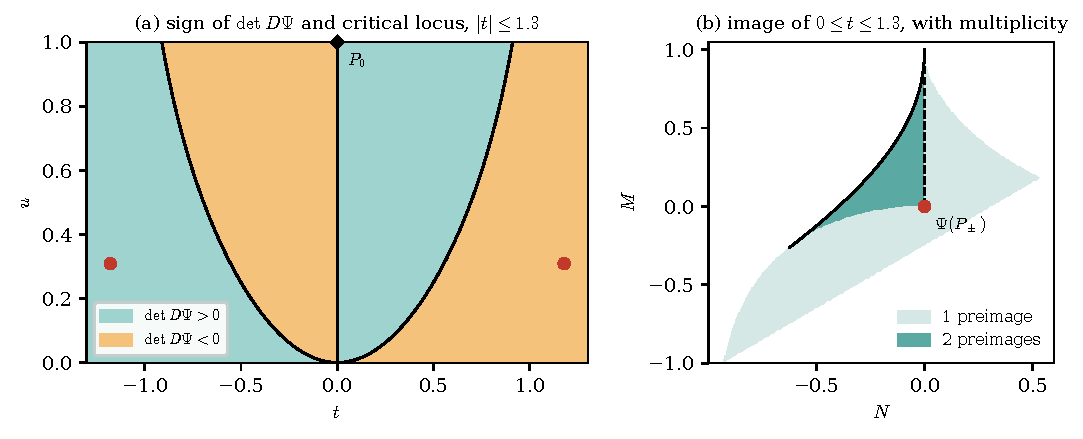
\includegraphics[width=\linewidth]{observation_folds.pdf}
\caption{The planar observation map $\Psi=(N,M)$. (a) The sign of
$\det D\Psi$ on $|t|\leq1.3$ and the critical locus: the symmetry segment $t=0$
and the rational branch through $(0,0)$. (b) Since $N$ and $M$ are even in $t$,
$\Psi(t,u)=\Psi(-t,u)$, so it suffices to draw the image of $0\leq t\leq1.3$.
The shading counts preimages in this half. The solid curve is the image of the
rational branch, the dashed segment that of $t=0$, and both lateral cross-caps
map to the origin. On $|t|\leq1.3$ every count doubles: for instance
$(N,M)=(-0.1,0.2)$ has the four preimages $(\pm0.9947,0.3375)$ and
$(\pm0.3687,0.7778)$.}\label{fig:folds}
\end{figure}

\subsection{Three sign structures}
\begin{proposition}[Carriers]\label{prop:carrier}
(1) For connected $X$, $\End_{D(X)}(\Z_X)=H^0(X;\Z)=\Z$. Every involution of
$\Z_X$ is therefore $\pm\mathrm{id}$, $\Z_X$ admits no splitting into two
nonzero summands, and its characteristic polynomial is $t-1$ or $t+1$. The same
holds for the constant condensed sheaf on a compact connected space, whose
global sections are the continuous maps to $\Z$.

(2) Let $X=D_\circ\setminus\{P_+,P_-,(0,1)\}$ and let $\pi:\widetilde X\to X$ be
the double cover $\{\chi^2=F\}$. Then $\pi_*\Z$ is a rank-two local system with
deck involution $\tau$, indecomposable over $\Z$. After inverting $2$,
$\pi_*\Z[\frac12]\simeq\Z[\frac12]\oplus\mathcal L[\frac12]$, where the sign
system $\mathcal L$ has monodromy $-1$ around each of $P_\pm$.

(3) The fold involution $(\xi,\eta)\mapsto(\xi,-\eta)$ and the deck involution
$\tau$ cannot be identified: the first fixes the fold arc, the second is free.

(4) For a standard cross-cap image $X'$ with topological normalization $\nu$,
the rational normalization defect
$\mathcal Q_\nu=\nu_*\Q_{\widetilde X'}/\Q_{X'}$ is $j_!\mathcal L_{\rm sgn}$,
the extension by zero of the sign line on the open double ray. Its stalk at the
pinch is zero, so every morphism from $\mathcal Q_\nu$ to a skyscraper at the
pinch vanishes.
\end{proposition}
\begin{proof}
(1) Degree-zero endomorphisms of a sheaf in degree zero are the global sections
of the sheaf $\mathcal{H}om(\Z,\Z)=\Z$, and a direct-sum splitting corresponds
to an idempotent. The only idempotents of $\Z$ are $0$ and $1$.

(2) $D_\circ\setminus\{(0,1)\}$ is star-shaped about an interior point, so
$\pi_1(X)$ is free on loops around $P_\pm$, on which $F$ winds $\mp1$. The
monodromy of $\pi$ is the surjection onto $C_2$, and the stalk of $\pi_*\Z$ is
the regular module $\Z[C_2]=\Z[x]/(x^2-1)$. Local systems correspond to
$\pi_1$-modules, so
\[
 \End(\pi_*\Z)\simeq\End_{\pi_1(X)}(\Z[C_2])=\End_{\Z[C_2]}(\Z[C_2])\simeq\Z[C_2],
\]
and direct-sum decompositions correspond to idempotents. If $(a+bx)^2=a+bx$,
then $b(2a-1)=0$, so $b=0$ and $a\in\{0,1\}$. Over $\Z[\frac12]$ the projectors
$(1\pm x)/2$ split the module.

(3) The fixed-point sets differ.

(4) Near the cross-cap, $\nu$ is the proper source map, with one preimage over
the pinch and off the double ray, and two preimages over the open double ray.
Proper base change gives $(\nu_*\Q)_p=\Q^{\nu^{-1}(p)}$. At one-preimage points
$\Q\to\Q$ is the identity, so the quotient stalk is $0$. At two-preimage points
the diagonal $\Q\to\Q^2$ has quotient $\Q$, through $(a,b)\mapsto a-b$, and
exchanging the sheets acts on it by $-1$. These stalk maps are compatible with
restriction. So $\mathcal Q_\nu$ restricts to the anti-invariant line on the
ray and vanishes at the pinch, which identifies it with $j_!\mathcal L_{\rm sgn}$
\cite{stacks}. Finally, $\Hom(\mathcal Q_\nu,i_*\Q)=\Hom(i^*\mathcal Q_\nu,\Q)=0$.
\end{proof}
The three structures are thus cleanly separated. The sign system $\mathcal L$
lives on the punctured source and records the winding of $F$; the normalization
line lives on the image double stratum and records the exchange of sheets; and
the constant sheaf carries no sign at all. Relating $\mathcal L$ to the
normalization line would require a new identification of these two
$\Z/2$-torsors, which would be a natural object to construct.

\subsection{Exceptional pullbacks and folds}
We use the six-functor formalism on finite-dimensional locally compact
Hausdorff spaces with $D(X)=D(\mathrm{Sh}(X;\Z))$ \cite[Ex.~5.9]{scholze},
$\omega_X=a_X^!\Z$ and $\mathbb D_X=\RHom(-,\omega_X)$. Three standard facts
are used:
\begin{itemize}
\item Verdier duality, $f^!\mathbb D_Y\simeq\mathbb D_Xf^*$
\cite[Prop.~4.6.9]{knp}, \cite[Ch.~III]{ks};
\item the stalk of $\omega_X$ at $x$ is the local homology $H_*(X,X\setminus x)$,
and $\omega_X\simeq\orr_X[n]$ on an $n$-manifold \cite[Rem.~4.6.19, Cor.~4.6.20]{knp};
\item open immersions satisfy $j^!=j^*$ and are cohomologically smooth
\cite[Rem.~5.4]{scholze}.
\end{itemize}
A map $f$ is cohomologically smooth when the comparison
$f^!\Z\otimes f^*(-)\to f^!(-)$ is an isomorphism, $f^!\Z$ is invertible, and
both properties persist under base change \cite[Def.~5.1]{scholze}.

\begin{theorem}[$f^!\Z$ depends only on the domain]\label{thm:shriek}
(1) For any continuous $f:X\to Y$ between topological manifolds without
boundary of dimensions $n$ and $m$, $f^!\Z_Y\simeq\orr_X\otimes f^*\orr_Y[n-m]$.

(2) Let $D'\subset\R^2$ be locally closed and convex with nonempty interior,
and let $j:\inte D'\to D'$ be the inclusion. For every continuous
$\Psi:D'\to\R^2$, $\Psi^!\Z\simeq j_!\Z_{\inte D'}$.
\end{theorem}
\begin{proof}
(1) Since $\omega_Y$ is invertible, $\Z_Y\simeq\mathbb D_Y\omega_Y$, so
$f^!\Z_Y\simeq\mathbb D_Xf^*\omega_Y=\RHom(f^*\orr_Y[m],\orr_X[n])$.

(2) If $x$ is not an interior point, then a point strictly between an interior
point and any point of $D'$ is interior. So $D'\setminus x$ is star-shaped,
hence contractible, and the local homology at $x$ vanishes. At interior points
it is $\Z[2]$. Therefore $\omega_{D'}\simeq j_!\Z_{\inte D'}[2]$, and
\[
 \Psi^!\Z_{\R^2}\simeq\Psi^!\mathbb D_{\R^2}(\Z_{\R^2}[2])
 \simeq\mathbb D_{D'}\Psi^*(\Z_{\R^2}[2])=\mathbb D_{D'}(\Z_{D'}[2])=\omega_{D'}[-2].
 \qedhere
\]
\end{proof}

\begin{corollary}\label{cor:shift}
For $\Psi$ of \eqref{eq:F} on $D_\circ$ and any inclusion $i:L\to D_\circ$, the
complex $i^*\Psi^!\Z$ is $\Z$ in degree $0$ on $L\cap\inte D_\circ$ and $0$ on
the sides $u=0,1$. In particular the formula $i^*\Psi^!\Z\simeq\Z[-1]$ stated
for the fold locus in the earlier public description holds at no point. For an
embedded open arc $L$ in the interior, $i^!\Psi^!\Z\simeq\orr_L[-1]$, a shift that
comes from the codimension of $L$.
\end{corollary}

\begin{proposition}[Where the fold is visible]\label{prop:detect}
Let $x$ be an interior ordinary fold point of $\Psi$, and choose disc
neighbourhoods $V\ni x$ and $W\ni\Psi(x)$ on which $f=\Psi|_V$ is homeomorphic
to $(\xi,\eta)\mapsto(\xi,\eta^2)$. Let $L$ be the fold arc, let $W'\subset W$
be the open side of the discriminant containing $f(V\setminus L)$, and put
$G=j'_!\Z_{W'}$. Then $f^!\Z_W\simeq\Z_V$, $f^*G\simeq(\Z_{V\setminus L})_!$ and
$f^!G\simeq\Z_V$. The comparison map $f^!\Z_W\otimes f^*G\to f^!G$ is injective
with cokernel $i_*\Z_L$. So at every ordinary fold point invertibility of
$f^!\Z$ holds, and the comparison condition is exactly what fails.
\end{proposition}
\begin{proof}
The first isomorphism is Theorem~\ref{thm:shriek}(1). Pullback commutes with
extension by zero and $f^{-1}(W')=V\setminus L$, which gives the second. For
the closed side $k:H\to W$, local homology vanishes on its edge, so
$\mathbb D_W(\Z_H)=k_*\omega_H\simeq G[2]$. Since $f(V)\subset H$, we get
$f^!G[2]\simeq\mathbb D_V(f^*\Z_H)=\mathbb D_V(\Z_V)=\Z_V[2]$.

Let $\phi:(\Z_{V\setminus L})_!\to\Z_V$ be the comparison map, read through
these identifications, and compute its kernel $\mathcal K$ and cokernel
$\mathcal C$ stalk by stalk. Off $L$, $f$ is locally an open immersion, so
$\phi$ is an isomorphism there, and $\mathcal K_y=\mathcal C_y=0$. On $L$ the
source stalk is $0$ and the target stalk is $\Z$, so $\mathcal K_y=0$ and
$\mathcal C_y=\Z$. Thus $\phi$ is injective and $\mathcal C$ is supported on
$L$. The surjection $\Z_V\to\mathcal C$ restricts to a surjection
$\Z_L\to i^*\mathcal C$, which is an isomorphism stalkwise, since a surjection
$\Z\to\Z$ is bijective. Hence $\mathcal C\simeq i_*\Z_L$.
\end{proof}
The fold also shows up in $f_*\Z_V$, whose stalk ranks are $2,1,0$ across the
discriminant, and on the surface side in the normalization defect. A compact
Hausdorff image defines a condensed set. The singularity information, however,
comes from the maps above rather than from the condensed structure itself
(v12 Remark~8.7).

\section{Residual geometry}\label{sec:residual}
\subsection{Sublevel law and resolution cost}
For the standard models take Lebesgue measure and the residuals
$K_f=x^2+y^4$ and $K_\times=x^2(1+y^2)+y^4$.
\begin{theorem}[Sublevel law]\label{thm:sublevel}
With $B=B(\frac14,\frac32)$ and $\varepsilon>0$,
\[
 V_f(\varepsilon)=B\varepsilon^{3/4},\qquad
 B\varepsilon^{3/4}(1+\sqrt\varepsilon)^{-1/2}\leq V_\times(\varepsilon)\leq B\varepsilon^{3/4}.
\]
The exponent $3/4$ is unchanged by smooth positive densities and by smooth
changes of source or target coordinates fixing the origin; the coefficient
may change.
\end{theorem}
\begin{proof}
Slicing in $y$ gives $4\int_0^{\varepsilon^{1/4}}\sqrt{\varepsilon-y^4}\dd y$.
Substituting $y=\varepsilon^{1/4}v$ and then $z=v^4$ yields $B\varepsilon^{3/4}$.
For the cross-cap, the extra factor $(1+y^2)^{-1/2}$ lies between
$(1+\sqrt\varepsilon)^{-1/2}$ and $1$.

The sublevel sets shrink to the origin, so a smooth positive density or the
Jacobian of a source diffeomorphism fixing $0$ is a positive constant plus
$o(1)$ on them, and $V$ is multiplied by a factor tending to a positive
constant. A target diffeomorphism fixing $0$ changes the squared residual by a
factor between positive constants $a\leq b$, so $V(\varepsilon/b)\leq V'(\varepsilon)\leq V(\varepsilon/a)$.
Neither change affects the exponent.
\end{proof}
The geometric resolution cost is therefore
$-\log V(\varepsilon)=\frac34\log\varepsilon^{-1}-\log B+o(1)$, a clean,
parameter-free law. A communication capacity is a different quantity: it
depends on a channel. For example, identical binary labels admit a constant
channel of capacity $0$ and a noiseless one of capacity $\log2$. Accordingly
the conjecture $C=\sqrt5\ln S$ from the earlier description is replaced by this
resolution law.

\begin{figure}[htb]\centering
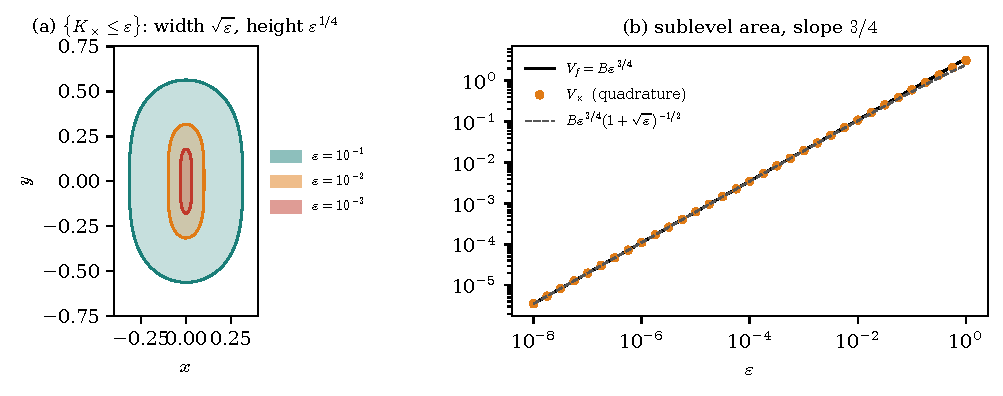
\includegraphics[width=\linewidth]{sublevel_law.pdf}
\caption{The sublevel law of Theorem~\ref{thm:sublevel}. (a) The sets
$\{K_\times\leq\varepsilon\}$ shrink anisotropically, with width
$\sqrt\varepsilon$ and height $\varepsilon^{1/4}$, so their area scales as
$\varepsilon^{1/2+1/4}$. (b) The cross-cap area, computed by quadrature,
between the two bounds of the theorem.}\label{fig:sublevel}
\end{figure}

\subsection{An explicitly chosen complex completion}
\begin{theorem}[Chosen $A_3$ completion]\label{thm:a3}
After its coefficients are extended to $\C$, the germ of $K_\times$ is
right-equivalent to $X^2+Y^4$, with Milnor and Tjurina numbers $3$. The fiber
$U=\{X^2+Y^4=1\}$ is a smooth genus-one curve $E$ with two points removed.
$H^1(U)$ has dimension three and monodromy spectrum $\{-i,1,i\}$. The weight-graded
pieces of its mixed Hodge structure have dimension two in weight one and one in
weight two.
\end{theorem}
\begin{proof}
The substitution $X=x\sqrt{1+y^2}$, $Y=y$ is a holomorphic coordinate change
with invertible derivative. The Milnor algebra is
$\C[X,Y]/(2X,4Y^3)$, of dimension $3$. By Euler's identity
$X^2+Y^4=\frac X2\cdot2X+\frac Y4\cdot4Y^3$ lies in the Jacobian ideal, so the
Tjurina number is also $3$. The weighted compactification
$X^2+Y^4=Z^4\subset\mathbb P(2,1,1)$ is a double cover of $\mathbb P^1$ branched
at four points, hence of genus one, and its two ends at infinity are
unramified. Weighted homogeneity identifies the global and local Milnor fibers
\cite{milnor,dimca}. The monodromy $h(X,Y)=(-X,iY)$ acts by $-i$ and $i$ on
$H^1(E)$ and fixes the boundary class. The Gysin sequence
$0\to H^1(E)\to H^1(U)\to\widetilde H^0(\{\infty_\pm\})(-1)\to0$ gives the
weights \cite{deligne,peters}.
\end{proof}
These Hodge-theoretic data belong to the chosen complexification. A full
nearby-cycle package would additionally need the specialization and variation
maps, which the monodromy alone does not determine.

\subsection{Three different projected curves}

\begin{figure}[htb]\centering
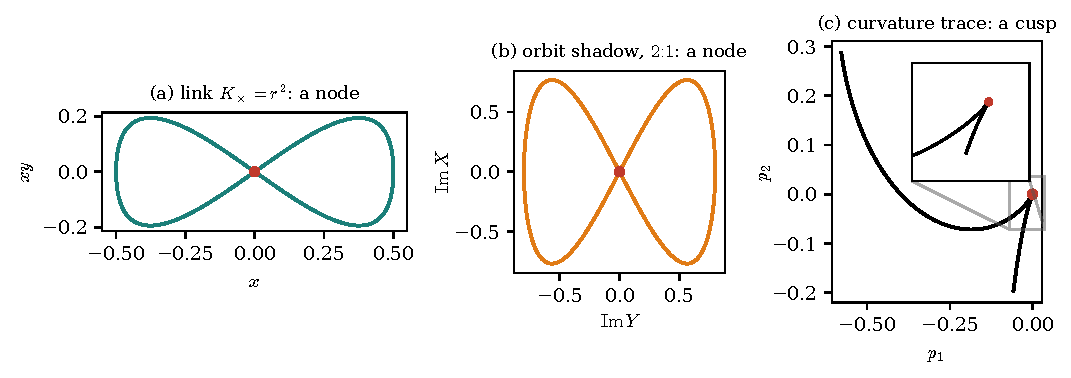
\includegraphics[width=\linewidth]{three_curves.pdf}
\caption{The three curves of Proposition~\ref{prop:curves}. (a) The image of the
real link $K_\times=r^2$ ($r=\frac12$), projected to the $(x,xy)$-plane; the
node is the double point $(0,0,r)$. (b) The shadow $(\Im Y,\Im X)$ of a weighted
orbit ($b=0.8$). (c) The pedal trace $p=(p_1,p_2)$ of the exceptional
principal curvature at the lateral cross-cap $P_+$, computed from the exact
invariants. The inset magnifies the ordinary cusp at the origin, where both
branches share one tangent.}\label{fig:curves}
\end{figure}

\begin{proposition}\label{prop:curves}
(1) For each $r>0$ the real link $\{K_\times=r^2\}$ is a circle whose cross-cap
image has one transverse double point, a figure-eight graph. The lift
$(x,xy,y^2,y)$ is an embedding.
(2) The weights of $X^2+Y^4$ are $(2,1)$. For $a,b>0$ with $a^2+b^4=1$, the orbit
$\Gamma(s)=(ae^{2is},be^{is})$ is embedded, and its shadow $(b\sin s,a\sin2s)$
is a transverse figure-eight with frequency ratio $2:1$. The action
$2\pi(4a^2+b^2)$ has infimum $2\pi$ over nondegenerate orbits, attained only in
their closure; $b^2=\frac18$ is a strict maximum.
(3) For the actual lateral germs the Euclidean Whitney invariants satisfy
$b_\pm^2+a_\pm c_\pm^2=0$, and the exceptional principal-curvature trace has an
ordinary cusp at its double return.
\end{proposition}
\begin{proof}
(1) The gradient of $K_\times$ vanishes only at $0$. Equal images force $x=x'$
and $y'=\pm y$, and the tangent images at $(0,\pm\sqrt r)$ are transverse.

(2) The $Y$ coordinate fixes the phase. With $z=b^2$, the action divided by $2\pi$
is $1+(1-z)(4z+3)$.

(3) Use the adapted pair $\xi=\partial_u/\sqrt3$ and
$\eta=-\partial_t+\lambda_\pm\partial_u$, where $\lambda_\pm=-c_0s_\pm/[2(1-c_0)]$.
Let $\Pi$ be the projection onto the normal plane of $S_u$, and put
$A=\Pi(S_{tt}-2\lambda_\pm S_{tu})$ and $B=\Pi(-S_{tu}/\sqrt3)$. The actual
second jet gives
\[
 |A|^2=\tfrac{-335+162\sqrt5}{12},\qquad
 \langle A,B\rangle^2=\tfrac{-520+249\sqrt5}{27},\qquad
 R=|B|^2-\tfrac{\langle A,B\rangle^2}{|A|^2}=\tfrac{20(140+11\sqrt5)}{11397}>0.
\]
Oriented Gram--Schmidt then gives
\[
 a=-\frac{\langle A,B\rangle^2}{2|A|^3},\qquad
 b_\pm=\pm\frac{\sqrt{\langle A,B\rangle^2R}}{|A|^2},\qquad
 c=\frac{\sqrt{2R}}{|A|^{1/2}},
\]
so $b^2+ac^2=0$ identically. In the Euclidean normal form the pedal trace is
\[
 p(\tau)=\frac{2(c\tau^2+2b\tau-ac)}{c^2+4\tau^2}\,(-c,2\tau)
\]
\cite[Prop.~2.1, Eq.~(2.8)]{principal}. Its numerator equals
$c(\tau-\tau_*)^2$ with $\tau_*=-b/c$, and
\[
 \det\bigl(p''(\tau_*),p'''(\tau_*)\bigr)=-\frac{96c^3}{(c^2+4b^2/c^2)^2}\neq0,
\]
which is the ordinary-cusp criterion.
\end{proof}
The three constructions produce three different curves, a node, a node and a
cusp, and each comes with its own data (Figure~\ref{fig:curves}).

\section{Open problems}\label{sec:open}
\begin{itemize}
\item Does a quadratic readout realize $S$ on $D_+$ under the original powers
(Remark~\ref{rem:data})? Is there a natural principle that selects a
non-analytic readout?
\item Construct a sign-twisted, differential-form or spinor operator whose boundary data
see the carriers of Proposition~\ref{prop:carrier}, and relate the phase sign
system to the normalization line.
\item The singular Dirac and Pin problem of v12 Sections~8.20--8.24. This
requires closed domains for the twisted Dirac operator of the actual Whitney
metric, graph and overlap estimates, singular-cut trace spaces, and
Clifford-compatible transmission maps. The exact-cone and regular-cut results
are the model cases. The scalar theory that serves as the first step is
developed in \cite{companion}.
\item Build signal or physical models in which capacity, mass, clocks or
chirality are defined independently, and compare them with the geometry above.
\end{itemize}

\appendix
\section{Review of the earlier record}\label{app:corrections}
\subsection{The public description}
The description field of the record \cite{record} shows the abstract of an
earlier draft, which differs from both public files. Its claims compare with
the present results as follows:
\begin{center}\small
\begin{tabular}{>{\raggedright\arraybackslash}p{.40\linewidth}>{\raggedright\arraybackslash}p{.52\linewidth}}\toprule
Claim in the description & Present status\\\midrule
$S$ is derived from the moment map and the power constraint & Not by analytic readouts (Theorem~\ref{thm:rigidity}); smooth realizations exist (Theorem~\ref{thm:smooth})\\
Immersion singularities occur at exactly two lateral points & Five rank labels (Proposition~\ref{prop:atlas})\\
Quasi-separated condensed set; Weil-étale/Pontryagin connection & Replaced by Bohr--Haar orthogonality (\S\ref{sec:spectral}) and Proposition~\ref{prop:carrier}(1)\\
$i^*\Psi^!\Z\simeq\Z[-1]$ on the fold locus & $\Psi^!\Z\simeq j_!\Z$ (Corollary~\ref{cor:shift}); folds seen by Proposition~\ref{prop:detect}\\
Monodromy as an endomorphism of the constant condensed sheaf & Carried by $\pi_*\Z$ (Proposition~\ref{prop:carrier})\\
$T>2(M-1)/\delta$ gives independence & Independence for all $T>0$ (\S\ref{sec:spectral})\\
$C=\sqrt5\ln S$ (conjectural) & Replaced by the $3/4$ resolution law (\S\ref{sec:residual})\\\bottomrule
\end{tabular}
\end{center}

\subsection{v11 Theorem 4.2}
v11 identified the sign reversal of $\sqrt F$ with an exchange of the sheets of
a Whitney fold; v12 dropped that identification, and
Proposition~\ref{prop:carrier}(3) shows why. In all other blocks up to 8.20,
v11 agrees with v12 apart from small refinements of wording. v11 stated the
spinorial parametrix as a remark, which matches the present open problem.

\subsection{All named statements of v12}
Categories: \textbf{H}~holds, possibly with an explicit domain or hypothesis;
\textbf{C}~holds after correction; \textbf{S}~strengthened; \textbf{R}~does
not hold as defined; \textbf{O}~open; \textbf{M}~model-level or conditional;
\textbf{D}~missing definition, settled here. ``C.'' refers to the companion
paper \cite{companion}, which proves the operator statements for general
surfaces with Whitney cross-caps; Section~9.2 of C.\ treats the present surface.
{\small
\begin{longtable}{@{}l>{\raggedright\arraybackslash}p{.06\linewidth}>{\raggedright\arraybackslash}p{.72\linewidth}@{}}
\toprule Block & Cat. & Note and location\\\midrule\endhead
3.1 & D & Analytic readouts excluded; smooth readout exists; other powers admit a quadratic readout (\S\ref{sec:realization})\\
3.2 & C & Fix $L^2(dx)$ and the conjugate-linear first slot; the introduction used another measure (\S\ref{sec:spectral})\\
3.3 & H & Geometric resolution cost (\S\ref{sec:residual})\\
4.1 & C & $F$ is an angular-chart field on $D_\circ$; indices $\mp1$ (\S\ref{sec:model}, Thm~\ref{thm:dipole})\\
4.2 & H & Two-traversal sign restoration (Thm~\ref{thm:dipole})\\
4.3 & H & Topological statement, as v12 says\\
4.4 & C & $N$ and $M$ are both even; corrected parity explanation (\S\ref{sec:monodromy})\\
5.1 & H & $|P'(c_0)|=\sqrt5$ for the monic $P$\\
5.2 & C & The lateral Jacobian modulus is about $2.245$; its sign follows the orientation\\
5.3 & H & Exact fold constant; two-sided cross-cap bounds (Thm~\ref{thm:sublevel})\\
5.4 & H & Uses an external identification $S=\varepsilon^{-1}$\\
5.5 & H & Capacity depends on a channel\\
5.6 & H & Explicit holomorphic coordinate change (Thm~\ref{thm:a3})\\
5.7 & H & Genus one, two unramified ends, spectrum $\{-i,1,i\}$\\
5.8 & H & Every $r>0$ for the standard model (Prop.~\ref{prop:curves})\\
5.9 & H & The orbit leaves the fixed fiber except at fourth-root phases\\
5.10 & C & Infimum attained only in the closure; $b^2=\frac18$ is a maximum\\
5.11 & H & Scope remark\\
5.12 & H & Invariants and cusp criterion (Prop.~\ref{prop:curves})\\
5.13 & H & Geometric no-go\\
6.1 & C & $c^2-3c+1$ selects the lateral labels; five rank labels (Prop.~\ref{prop:atlas})\\
6.2 & C & Five cross-cap germs, including two corner quarter-germs\\
7.1 & C & Formal adjoint parameter depends on the measure; domains made explicit\\
7.2 & H & Indices $(1,0)$ with explicit $H^1_0$ and $H^1$ domains\\
7.3 & C & For $\sigma>\frac12$ the functions are $L^2$ with nonzero trace\\
7.4 & H & Conventions made explicit\\
7.5 & H & For a fixed finite family\\
7.6 & S & Independence for every $T>0$; the threshold controls conditioning\\
7.7 & H & Bohr torus realization\\
7.8 & H & Conditioning and log-determinant bounds\\
8.1 & H & Full-line and half-line realizations distinguished\\
8.2 & H & Evaluation boundary $\sigma=\frac12$\\
8.3 & H & Two separate thresholds\\
8.4 & H & Character orthogonality\\
8.5 & H & Lattices of lower rank retained\\
8.6 & H & Normalization defect (Prop.~\ref{prop:carrier}(4))\\
8.7 & H & Sharpened by Thm~\ref{thm:shriek}\\
8.8 & C & Fold proved through exact charts; remainder term added (Prop.~\ref{prop:polar})\\
8.9 & C & All five labels removed; $H_1=\Z^2$\\
8.10 & H & On finite-energy conforming spaces, $J_n^*G_{n+1}J_n=G_n$ and $J_n^*K_{n+1}J_n=K_n$ follow from sesquilinearity, since $\varphi^{(n)}_i=\sum_\alpha(J_n)_{\alpha i}\varphi^{(n+1)}_\alpha$; no convergence is claimed\\
8.11 & C & Closures are form closures. Zero capacity holds at $P_\pm$ (C.\ Prop.~4.1), and at $P_0$, $E_\pm$ by restricting the same cutoffs to the physical germ\\
8.12 & O & The model identities hold; the uniform estimate for the actual germ is unproved. It is not needed: arclength coordinates make the metric uniformly elliptic (C.\ Lemma~3.2)\\
8.13 & R & The graph closure of the interior core has infinite deficiency from the outer boundary (C.\ Prop.~8.1). The corrected operator $H_F|_{\ker\tau}$ has indices $(2,2)$ and the stated logarithmic boundary form (C.\ Thms.~5.2, 6.1, 6.3)\\
8.14 & R & Fails for the old minimum, which has a Neumann extension (C.\ Prop.~8.1); holds for the corrected operator (C.\ Cors.~7.1, 7.2)\\
8.15 & R & Compactness and the gap hold (C.\ Thm.~4.2). The Krein kernel of the old minimum is infinite-dimensional (C.\ Prop.~8.1); that of the corrected operator is two-dimensional (C.\ Thm.~5.2)\\
8.16 & H & For the actual $H_0$: strictly positive, with Friedrichs extension $H_F$, discrete reduced Krein spectrum and the weak buckling equivalence (C.\ Prop.~8.1)\\
8.17 & C & Operator scope: the fixed-boundary Friedrichs operator and its point restriction (C.\ \S\S4--7)\\
8.18 & H & Support and parity obstruction (Prop.~\ref{prop:carrier})\\
8.19 & H & Scope remark\\
8.20 & M & Exact-cone model (\S\ref{sec:open})\\
8.21 & O & Actual front--seam parametrix (\S\ref{sec:open})\\
8.22 & M & First-order data hold; a Pin convention must be chosen\\
8.23 & M & Conditional on a Clifford-compatible transmission\\
8.24 & H & Open-problem statement\\
8.25 & H & For a specified proper lift (\S\ref{sec:limits})\\
8.26 & H & Representation observation\\
8.27 & H & Real-geometry Deligne/Weil scope\\
8.28 & H & Weights of the chosen completion (Thm~\ref{thm:a3})\\
8.29 & H & Monodromy versus the full nearby-cycle package\\
8.30 & H & For a specified Weil realization\\
9.1 & H & The ratio is a length\\
9.2 & H & Numerical pattern\\
9.3 & H & Power coordinates Poisson-commute\\
9.4 & H & A separate observable programme\\
9.5 & H & $\eta=0$ for the sign circle\\
9.6 & H & Sign cover and spectral symmetry\\\bottomrule
\end{longtable}}

\section{Spectral and arithmetic estimates}\label{sec:spectral}
The earlier versions used the following classical facts. We collect them in
the precise form the model uses; they are independent of the realization and
monodromy results of the main text.

\paragraph{Mellin operators.} Let $T_\sigma f=-i(xf'+\sigma f)$. For $C^1$
functions on $[a,b]\subset(0,\infty)$,
$\int_a^b(\overline{T_\sigma f}g-\overline fT_{1-\sigma}g)\dd x=i[x\overline fg]_a^b$.
In $L^2(dx)$ the formal adjoint is therefore $T_{1-\sigma}$, which equals
$T_\sigma$ exactly at $\sigma=\frac12$; for the measure $x^{2\beta-1}\dd x$ the
parameter becomes $2\beta-\sigma$. The map $(Uf)(s)=e^{s/2}f(e^s)$ is unitary from
$L^2([1,\infty),dx)$ onto $L^2([0,\infty),ds)$. It carries the closure of
$T_{1/2}$ on $C_c^\infty$ to $-i\partial_s$ on $H^1_0$, whose adjoint has domain
$H^1$. The deficiency indices are $(1,0)$, so the half-line operator has no
self-adjoint extension, while on the full multiplicative line it is
self-adjoint \cite{reed}. The functions $x^{-\sigma-i\omega}$ satisfy
$T_\sigma x^{-\sigma-i\omega}=-\omega x^{-\sigma-i\omega}$. They are generalized
eigenfunctions at $\sigma=\frac12$, and for $\sigma>\frac12$ they are square-integrable
but have nonzero trace at $x=1$.

\paragraph{Finite Gram matrices.} For distinct real $\omega_1,\dots,\omega_M$,
$T>0$ and $G_{jk}=T^{-1}\int_0^Te^{i(\omega_j-\omega_k)t}\dd t$, the phasors are
linearly independent and $G$ is positive definite for \emph{every} $T>0$. Indeed,
a vanishing combination and its first $M-1$ derivatives at an interior time give
a Vandermonde system. With $\varepsilon=2(M-1)/(T\min|\omega_j-\omega_k|)<1$, the
spectrum of $G$ lies in $[1-\varepsilon,1+\varepsilon]$,
$\kappa_2(G)\leq(1+\varepsilon)/(1-\varepsilon)$ and
$M\log(1-\varepsilon)\leq\log\det G\leq0$. The threshold $T>2(M-1)/\delta$ of the
earlier versions therefore quantifies conditioning.

\paragraph{Hardy evaluation and Bohr--Haar.} On the coefficient Hilbert space
of Dirichlet series, evaluation at $\Re s=\sigma$ is bounded exactly when
$\sigma>\frac12$, with norm $\zeta(2\sigma)^{1/2}$ \cite{hardy}. The Gram limit
$\lim T^{-1}\int_0^Tn^{it}m^{-it}\dd t=\delta_{nm}$ is character orthogonality on
the product torus of prime exponents. That torus also records relations: a
finite set of integers may generate a lattice of lower rank, as $\{2,4\}$ does.

\begin{proposition}[Log-scale and linear-scale windows]\label{prop:windows}
Let $K(\delta,L)=L^{-1}\int_0^Le^{-i\delta\tau}\dd\tau$, so that
$|K|=|\sin(\delta L/2)|/(|\delta|L/2)\leq2/(|\delta|L)$, and let $T>1$.
\begin{enumerate}
\item $\frac1{\log T}\int_1^Tx^{-i\delta}\frac{dx}x=K(\delta,\log T)$. The
log-scale and linear-scale bounds are the single bound $2/(|\delta|\cdot\text{mass})$
evaluated at window masses $\log T$ and $T$, for every real $\delta$.
\item With Lebesgue measure on the same interval,
$\frac1{T-1}\int_1^Tx^{-i\delta}\dd x=\frac{T^{1-i\delta}-1}{(1-i\delta)(T-1)}$,
whose modulus tends to $(1+\delta^2)^{-1/2}$.
\item For $e^{-i\delta t}$ on $[1,T]$ with Haar measure, the average is at most
$2/(|\delta|\log T)$ in modulus.
\end{enumerate}
\end{proposition}
\begin{proof}
Substitute $x=e^\tau$; integrate directly; integrate by parts once.
\end{proof}
So the two rates compare window masses, $T$ against $\log T$, and the
characters of $(\R_{>0},\times)$ decorrelate under Haar measure but not under
Lebesgue measure. This replaces the integer-sparsity explanation given in the
earlier description; note also that the positive integers generate the dense
subgroup $\Q_{>0}$.

\section{Scope statements carried over}\label{sec:limits}
The following statements of v12 hold as stated there:
\begin{itemize}
\item A nonempty proper subset of $SU(2)$ is not invariant under the full left
action. This applies to a constrained source lift once one is specified.
\item The ratio $2\pi^2R^3/(\pi r^2)$ with $r=\phi^{-2}R$ equals $2\pi\phi^4R$.
It is a length, so a mass law would need its own scale and operator.
\item For the canonical Kähler form the two power coordinates Poisson-commute.
The full $SU(2)$ moment map generates a noncommutative algebra and is a natural
starting point for quantization.
\item The antiperiodic circle operator $-i\partial_\theta$ has the symmetric
spectrum $\Z+\frac12$ and vanishing eta invariant \cite{aps}.
\item The pair $(E,D)$ of Theorem~\ref{thm:a3} can be evaluated by any Weil
cohomology theory with localization and Tate twists, giving a one-dimensional
boundary term; such a theory is an additional choice.
\end{itemize}

\section{Evidence and reproducibility}\label{app:evidence}
The historical authority is the public v12 file, which is byte-identical to
the archived copy. The SHA-256 values of the two public files are
\begin{center}\footnotesize
\begin{tabular}{@{}ll@{}}
v12 & \texttt{4ebb8f0a7d6e88a6c5cd97f65d224b4e938867cabad54f057d3ceafb24167d5a}\\
v11 & \texttt{207a51feed62fe7f5a6dd7c9190258dd1b9c996c8b2735e799aff569bb017ec2}
\end{tabular}
\end{center}

All proofs are given in full in the text. The figures are generated by a
script from the explicit formulas of the paper; their numerical panels
illustrate results proved in the text.

\paragraph{Exact and finite replay.} Independent scripts check the following:
\begin{itemize}
\item the derivative determinants, the Euclidean jet invariants of
Proposition~\ref{prop:curves}(3) and the polar remainder;
\item the quadrature and Bloch identities;
\item the edge and skew-line algebra;
\item a replay of the $C^\infty$ readout on $801\times81$ source labels, which
reproduces $S$ to $1.4\times10^{-14}$;
\item the analytic edge-chart identities on the half source;
\item the Jacobian factorization, the windings $\mp1$ and the idempotents of
$\Z[C_2]$;
\item the window kernels.
\end{itemize}
They confirm the algebra the written proofs rely on.

\paragraph{Lean.} A companion Lean project (Lean~4, Mathlib) contains 33 named
theorems, audited for proof holes and custom axioms. They include:
\begin{itemize}
\item the actual rank classification, the endpoint ranks and the polar fold;
\item the small-circle indices and the evenness of the field;
\item the monic derivative;
\item the injectivity and fibres of the cross-cap lift;
\item square-root and logarithm lifting;
\item the Mellin interval identity, and the Gram entries with their eigenvalue
enclosure;
\item the quadrature readout identities and the cusp factorization.
\end{itemize}
This is partial coverage of selected statements.

\paragraph{External theorems.} The following external results are used, each
with its hypotheses verified for the actual maps:
\begin{itemize}
\item smooth cross-cap recognition \cite{hasegawa};
\item the real-analytic inverse function theorem \cite{krantzparks};
\item Milnor fiber comparison and mixed Hodge theory \cite{milnor,dimca,deligne,peters};
\item the Euclidean pedal formula \cite{principal};
\item Verdier duality and six-functor smoothness \cite{knp,scholze,ks};
\item Dirichlet--Hardy space facts \cite{hardy};
\item self-adjointness by Fourier transform \cite{reed}.
\end{itemize}

{\small
\begin{thebibliography}{99}
\bibitem{record} A. Hayami (J.-Y. Huang), \emph{Geometric Realization of Bicomplex
Signal Manifolds: Spectral Stability, Whitney Folds, and Monodromy of the
Observation Field}, preprint, ResearchGate, 2026, files v11 and v12.
\href{https://doi.org/10.13140/RG.2.2.17048.15361}{doi:10.13140/RG.2.2.17048.15361}.
\bibitem{ruled} A. Hayami, \emph{The Orthogonal-Circle Ruled Surface: A Boundary
Atlas, Five Rank Singularities, and Conditional Fold-Signal Recurrence}, 2026.
\href{https://doi.org/10.5281/zenodo.23073642}{doi:10.5281/zenodo.23073642}.
\bibitem{stokes} A. Hayami, \emph{Observation Discriminant and Spherical Fold Image
of the Orthogonal-Circle Ruled Surface}, 2026.
\href{https://doi.org/10.5281/zenodo.22728902}{doi:10.5281/zenodo.22728902}.
\bibitem{companion} A. Hayami, \emph{Pseudo-Laplacians at Whitney Cross-Caps:
Point Interactions on Surfaces Mapped into Three-Space}, in preparation.
\bibitem{hasegawa} M. Hasegawa et al., \emph{Intrinsic properties of surfaces
with singularities}, \href{https://arxiv.org/abs/1409.0281}{arXiv:1409.0281}, \S4.
\bibitem{bloch} K. Szyma\'nski and K. \.Zyczkowski, \emph{Geometric and algebraic
origins of additive uncertainty relations}, arXiv:1804.06191, \S II.
\bibitem{krantzparks} S. G. Krantz and H. R. Parks, \emph{A Primer of Real
Analytic Functions}, 2nd ed., Birkh\"auser, 2002.
\bibitem{scholze} P. Scholze, \emph{Six-Functor Formalisms}, lecture notes,
\href{https://arxiv.org/abs/2510.26269}{arXiv:2510.26269v2}, Def.~5.1, Rem.~5.4, Ex.~5.9.
\bibitem{knp} A. Krause, T. Nikolaus and P. P\"utzst\"uck, \emph{Sheaves on
Manifolds}, lecture notes, 2024, \S4.6.
\bibitem{ks} M. Kashiwara and P. Schapira, \emph{Sheaves on Manifolds},
Springer, 1990, Ch.~III.
\bibitem{stacks} The Stacks Project Authors, Tag 009Z.
\bibitem{milnor} J. Milnor, \emph{Singular Points of Complex Hypersurfaces},
Princeton University Press, 1968.
\bibitem{dimca} A. Dimca, \emph{Singularities and Topology of Hypersurfaces},
Springer, 1992.
\bibitem{deligne} P. Deligne, Th\'eorie de Hodge II, \emph{Publ. Math. IHES}
40 (1971), 5--57.
\bibitem{peters} C. Peters and J. Steenbrink, \emph{Mixed Hodge Structures},
Springer, 2008.
\bibitem{principal} L. F. Martins, K. Saji, S. P. dos Santos and R. Shimada,
\emph{Geometry on principal curvature surfaces},
\href{https://arxiv.org/abs/2607.21796}{arXiv:2607.21796}, Prop.~2.1.
\bibitem{reed} M. Reed and B. Simon, \emph{Methods of Modern Mathematical
Physics I}, Academic Press, 1972.
\bibitem{hardy} H. Hedenmalm, P. Lindqvist and K. Seip, A Hilbert space of
Dirichlet series and systems of dilated functions in $L^2(0,1)$,
\emph{Duke Math. J.} 86 (1997), 1--37.
\bibitem{aps} M. F. Atiyah, V. K. Patodi and I. M. Singer, Spectral asymmetry
and Riemannian geometry I, \emph{Math. Proc. Cambridge Philos. Soc.} 77 (1975), 43--69.
\end{thebibliography}}
\end{document}
